\chapter{Exodus 40}

\begin{figure}
  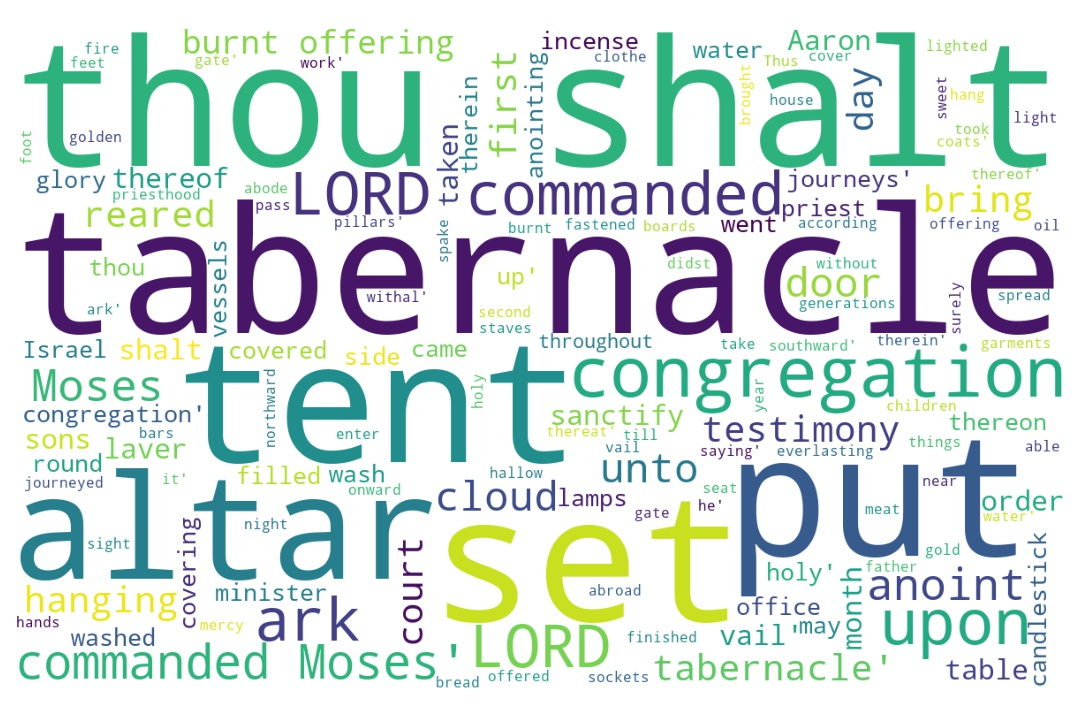
\includegraphics[width=\linewidth]{02OT-Exodus/Exodus40-WordCloud.jpg}
  \caption{Exodus 40 Word Cloud}
  \label{fig:Exodus 40 word Cloud}
\end{figure}


\marginpar{\scriptsize \centering \fcolorbox{bone}{lime}{\textbf{TABERNACLE: IOC}}\\ (Exodus 40:1-38) \begin{compactenum}[I.][8]
    \item \textbf{New Year's Day} \index[scripture]{Exodus!Exo 40:02}(Exo 40:2)  
    \item \textbf{Anointing} \index[scripture]{Exodus!Exo 40:09}\index[scripture]{Exodus!Exo 40:10}\index[scripture]{Exodus!Exo 40:11}\index[scripture]{Exodus!Exo 40:13}\index[scripture]{Exodus!Exo 40:15}(Exo 40:9, 10, 11, 13, 15) 
    \item \textbf{Needed Items} (the furniture of the tabernacle)  
    \item The \textbf{Nearness of God} \index[scripture]{Exodus!Exo 39:34}\index[scripture]{Exodus!Exo 39:35}\index[scripture]{Exodus!Exo 39:36}\index[scripture]{Exodus!Exo 39:37}\index[scripture]{Exodus!Exo 39:38}(Exo 39:34, 35, 36, 37, 38)  (the cloud)
    \item \textbf{Necessary Staff} \index[scripture]{Exodus!Exo 39:30--33}(Exo 39:30--33)  
    \item The \textbf{Numbers} 
    \begin{compactenum}[A.]
        \item The word ``tabernacle'' is used 18 times in chapter (number of bondage)
        \item The word ``Moses'' is used 13 times in chapter (number of rebellion)
    \end{compactenum}
\end{compactenum}}





\footnote{\textcolor[cmyk]{0.99998,1,0,0}{\hyperlink{TOC}{Return to end of Table of Contents.}}}\footnote{\href{https://audiobible.com/bible/exodus_40.html}{\textcolor[cmyk]{0.99998,1,0,0}{Exodus 40 Audio}}}\textcolor[cmyk]{0.99998,1,0,0}{And the LORD spake unto \fcolorbox{bone}{bone}{Moses}, saying,}
[2] \textcolor[cmyk]{0.99998,1,0,0}{On the \fcolorbox{bone}{lime}{first day} of the \fcolorbox{bone}{lime}{first month} shalt thou set up the tabernacle of the \fcolorbox{bone}{bone}{tent} of the congregation.}
[3] \textcolor[cmyk]{0.99998,1,0,0}{And thou shalt \fcolorbox{bone}{bone}{put} therein the ark of the testimony, and cover the ark with the vail.}
[4] \textcolor[cmyk]{0.99998,1,0,0}{And thou shalt bring in the table, and set in order the things that are to be set in order upon it; and thou shalt bring in the candlestick, and light the lamps thereof.}
[5] \textcolor[cmyk]{0.99998,1,0,0}{And thou shalt set the altar of gold for the incense before the ark of the testimony, and \fcolorbox{bone}{bone}{put} the hanging of the door to the tabernacle.}
[6] \textcolor[cmyk]{0.99998,1,0,0}{And thou shalt set the altar of the burnt offering before the door of the tabernacle of the \fcolorbox{bone}{bone}{tent} of the congregation.}
[7] \textcolor[cmyk]{0.99998,1,0,0}{And thou shalt set the laver between the \fcolorbox{bone}{bone}{tent} of the congregation and the altar, and shalt \fcolorbox{bone}{bone}{put} water therein.}
[8] \textcolor[cmyk]{0.99998,1,0,0}{And thou shalt set up the court round about, and hang up the hanging at the court gate.}
[9] \textcolor[cmyk]{0.99998,1,0,0}{And thou shalt take the \fcolorbox{bone}{lime}{anointing oil}, and anoint the tabernacle, and all that \emph{is} therein, and shalt hallow it, and all the vessels thereof: and it shall be holy.}
[10] \textcolor[cmyk]{0.99998,1,0,0}{And thou shalt anoint the altar of the burnt offering, and all his vessels, and sanctify the altar: and it shall be an altar most holy.}
[11] \textcolor[cmyk]{0.99998,1,0,0}{And thou shalt anoint the laver and his foot, and sanctify it.}
[12] \textcolor[cmyk]{0.99998,1,0,0}{And thou shalt bring Aaron and his sons unto the door of the tabernacle of the congregation, and wash them with water.}
[13] \textcolor[cmyk]{0.99998,1,0,0}{And thou shalt \fcolorbox{bone}{bone}{put} upon Aaron the holy garments, and anoint him, and sanctify him; that he may minister unto me in the priest's office.}
[14] \textcolor[cmyk]{0.99998,1,0,0}{And thou shalt bring his sons, and clothe them with coats:}
[15] \textcolor[cmyk]{0.99998,1,0,0}{And thou shalt anoint them, as thou didst anoint their father, that they may minister unto me in the priest's office: for their anointing shall surely be an everlasting priesthood throughout their generations.}
[16] \textcolor[cmyk]{0.99998,1,0,0}{Thus did \fcolorbox{bone}{bone}{Moses}: according to all that the LORD commanded him, so did he.}\\
\\
\P \textcolor[cmyk]{0.99998,1,0,0}{And it came to pass in the first month in the second year, on the first \emph{day} of the month, \emph{that} the tabernacle was reared up.}
[18] \textcolor[cmyk]{0.99998,1,0,0}{And \fcolorbox{bone}{bone}{Moses} reared up the tabernacle, and fastened his sockets, and set up the boards thereof, and \fcolorbox{bone}{bone}{put} in the bars thereof, and reared up his pillars.}
[19] \textcolor[cmyk]{0.99998,1,0,0}{And he spread abroad the \fcolorbox{bone}{bone}{tent} over the tabernacle, and \fcolorbox{bone}{bone}{put} the covering of the \fcolorbox{bone}{bone}{tent} above upon it; as the LORD commanded \fcolorbox{bone}{bone}{Moses}.}\\
\\
\P \textcolor[cmyk]{0.99998,1,0,0}{And he took and \fcolorbox{bone}{bone}{put} the testimony into the ark, and set the staves on the ark, and \fcolorbox{bone}{bone}{put} the mercy seat above upon the ark:}
[21] \textcolor[cmyk]{0.99998,1,0,0}{And he brought the ark into the tabernacle, and set up the vail of the covering, and covered the ark of the testimony; as the LORD commanded \fcolorbox{bone}{bone}{Moses}.}\\
\\
\P \textcolor[cmyk]{0.99998,1,0,0}{And he \fcolorbox{bone}{bone}{put} the table in the \fcolorbox{bone}{bone}{tent} of the congregation, upon the side of the tabernacle northward, without the vail.}
[23] \textcolor[cmyk]{0.99998,1,0,0}{And he set the bread in order upon it before the LORD; as the LORD had commanded \fcolorbox{bone}{bone}{Moses}.}\\
\\
\P \textcolor[cmyk]{0.99998,1,0,0}{And he \fcolorbox{bone}{bone}{put} the candlestick in the \fcolorbox{bone}{bone}{tent} of the congregation, over against the table, on the side of the tabernacle southward.}
[25] \textcolor[cmyk]{0.99998,1,0,0}{And he lighted the lamps before the LORD; as the LORD commanded \fcolorbox{bone}{bone}{Moses}.}\\
\\
\P \textcolor[cmyk]{0.99998,1,0,0}{And he \fcolorbox{bone}{bone}{put} the golden altar in the \fcolorbox{bone}{bone}{tent} of the congregation before the vail:}
[27] \textcolor[cmyk]{0.99998,1,0,0}{And he burnt sweet incense thereon; as the LORD commanded \fcolorbox{bone}{bone}{Moses}.}\\
\\
\P \textcolor[cmyk]{0.99998,1,0,0}{And he set up the hanging \emph{at} the door of the tabernacle.}
[29] \textcolor[cmyk]{0.99998,1,0,0}{And he \fcolorbox{bone}{bone}{put} the altar of burnt offering \emph{by} the door of the tabernacle of the \fcolorbox{bone}{bone}{tent} of the congregation, and offered upon it the burnt offering and the meat offering; as the LORD commanded \fcolorbox{bone}{bone}{Moses}.}\\
\\
\P \textcolor[cmyk]{0.99998,1,0,0}{And he set the laver between the \fcolorbox{bone}{bone}{tent} of the congregation and the altar, and \fcolorbox{bone}{bone}{put} water there, to wash \emph{withal}.}
[31] \textcolor[cmyk]{0.99998,1,0,0}{And \fcolorbox{bone}{bone}{Moses} and Aaron and his sons washed their hands and their feet thereat:}
[32] \textcolor[cmyk]{0.99998,1,0,0}{When they went into the \fcolorbox{bone}{bone}{tent} of the congregation, and when they came near unto the altar, they washed; as the LORD commanded \fcolorbox{bone}{bone}{Moses}.}
[33] \textcolor[cmyk]{0.99998,1,0,0}{And he reared up the court round about the tabernacle and the altar, and set up the hanging of the court gate. So \fcolorbox{bone}{bone}{Moses} finished the work.}\\
\\
\P \textcolor[cmyk]{0.99998,1,0,0}{Then \fcolorbox{bone}{lime}{a cloud} covered the \fcolorbox{bone}{bone}{tent} of the congregation, and the glory of the LORD filled the tabernacle.}
[35] \textcolor[cmyk]{0.99998,1,0,0}{And \fcolorbox{bone}{bone}{Moses} was not able to enter into the \fcolorbox{bone}{bone}{tent} of the congregation, because \fcolorbox{bone}{lime}{the cloud} abode thereon, and the glory of the LORD filled the tabernacle.}
[36] \textcolor[cmyk]{0.99998,1,0,0}{And when \fcolorbox{bone}{lime}{the cloud} was taken up from over the tabernacle, the children of Israel went onward in all their journeys:}
[37] \textcolor[cmyk]{0.99998,1,0,0}{But if \fcolorbox{bone}{lime}{the cloud} were not taken up, then they journeyed not till the day that it was taken up.}
[38] \textcolor[cmyk]{0.99998,1,0,0}{For \fcolorbox{bone}{lime}{the cloud} of the LORD \emph{was} upon the tabernacle by day, and fire was on it by night, in the sight of all the house of Israel, throughout all their journeys.}